\section{Performance}
\label{performance}

In this section, we discuss the real-world performance obtained by running the SIFT detection algorithm as described in section~\ref{sift} and the neural network as described in section~\ref{neural_network}. We chose a relatively old, mid-range laptop to run the tests on as it was the machine that we intended to use for our demo during the poster session. The laptop was a 2012 Macbook equipped with a <CPU>, <RAM>, <GFX>, running on <MAC OS darwin???>.

\subsection{SIFT}

\begin{table}[t]
\caption{SIFT Ratios Matches}
\label{sift_ratios}
\begin{center}
\begin{tabular}{ll}
\multicolumn{1}{c}{\bf RATIO}  &\multicolumn{1}{c}{\bf INCORRECT MATCHES}
\\ \hline \\
0.50             &111 of 196 \\
0.60             &105 of 196 \\
0.70             &100 of 196 \\
0.72             &95 of 196 \\
0.74             &95 of 196 \\
0.76             &91 of 196 \\
0.78             &94 of 196 \\
0.80             &98 of 196 \\
0.90             &102 of 196 \\
\end{tabular}
\end{center}
\end{table}

[WIP] The SIFT gesture detector was able to run in real-time, although it only had an accuracy of 53.57\%.

\subsection{Neural Network}
Out of all the networks, network7 performed the best with 100\% training accuracy and 90\% test accuracy.

\begin{figure}[h]
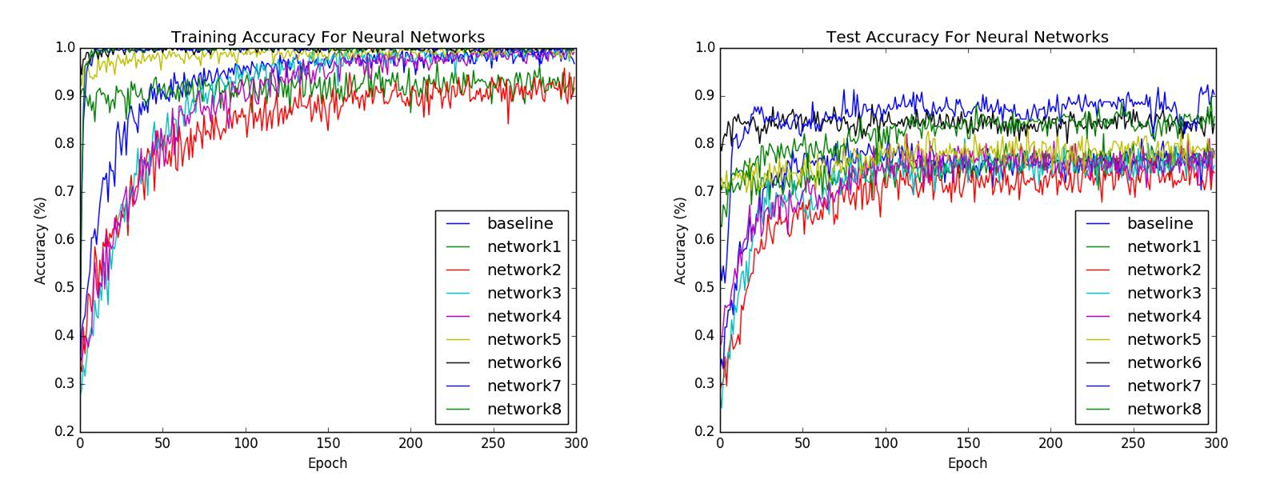
\includegraphics[scale=0.35]{accuracy.png}
\centering
\caption{Training and test accuracy of all the neural networks}
\end{figure}